
\lfoot{Autor: Fitim Faiku}
\subsubsection{Grundsätze einer Android Applikation}
\label{subsec:aapp-fundam}

Android Apps werden in der Programmiersprache Java geschrieben.
Die Android SDK-Tools kompilieren Code zusammen mit allen Ressourcen-Dateien in eine APK.
Eine APK ist ein Android-Paket, welches alle Inhalte einer Android App enthält. 
Die APK-Datei wird dann auf das Android-Gerät installiert. 


\textbf{Native vs HTML5 vs Hybrid} \newline
Bei der Umsetzung unserer Android Applikation, hatten wir die Entscheidung, wie wir die Android App erstellen. 
Da Android mehrere Programmierarten unterstützt musste evaluiert werden welche Programmiermodule für unsere App am besten geeignet ist. \nextline

\textbf{Native\newline} 
Der Vorteil an Native Apps ist, das sie auf die Hardware wie z.B. Kamera und GPS zugriff haben. 
Weiterhin ist der Verkauf nicht sehr schwer, da es auf Appstore draufgeladen werden kann. 
Für native Apps wird auf der Android-Plattform die Sprache Java verwendet.
Native Apps zeigen die beste Performance.
Die Dokumentation zu Nativen Apps ist am besten, da es über 2500 Bücher zur Android Entwicklung gibt.
Für nativ Apps werden Entwicklungsumgebungen-IDE(Integrated Developement Enviroment) verwendet um die gewünschte App zu Programmieren.\nextline


\textbf{HTML5\newline} 
Da eine HTML 5 Applikation über den Webbrowser laufen kann, sind die Entwickler nicht von AppStore oder anderen Plattformen abhängig. 
HTML5 verwendet Standard Web Technologien, wie JavaScript und CSS.
HTML5 Applikationen werden über Browser abgespielt, wobei jedes Gerät auf die Browser zugreifen kann und dadurch die App auf mehreren Plattformen abgespielt werden kann. \nextline

\textbf{Hybrid\newline} 
Hybrid Apps sind eine Mischung aus nativ und HTML5 Apps. Hybrid bietet das Beste aus beiden Welten. Das Design wird mittels HTML5 und CSS erstellt, wobei sich dahinter ein JavaScript-Code befindet. Hybrid Apps sind genauso auf jede Plattform abspielbar, wobei sie für die Plattform entsprechend umprogrammiert müssten.    
\nextline

\subsubsection{Android Virtual Device}
Ein Android Virtual Device(AVD) ist eine Emulator-Konfiguration, welche benutzt werden kann, um die Handysoftware darzustellen. 
Der einfachste Weg, um ein AVD zu schaffen, ist, den AVD-Manager in Android-Studio zu nutzen. 
Es kann auch auf performantere AVDs zugegriffen werden, um damit optimierte Applikationen zu schreiben.
Diese externen AVDs bieten eine realitätsnahe Darstellung des verwendeten Devices.
Zum Verwenden der AVD müssen System-image Packages runter geladen werden, wodurch die Software der AVD zugeordnet wird und mit verschiedenen API Versionen gearbeitet werden kann.
Eine API(Application Programming Interface) ist die Version der Programmierstelle, wobei mehrere Feauters auf höheren Versionen möglich sind. 
Eine Zuordnung zu einem System-Image: Sie können festlegen, welche Version der Android-Plattform auf dem virtuellen Gerät ausgeführt werden. Sie können eine Version der Standard-Android-Plattform oder das System-Image mit einem SDK Add-on verpackt wählen.

Es können so viele AVDs erstellt werden, basierend auf das Devicetypen mit denen man arbeiten möchte.
Beachten Sie folgende Punkte, wenn sie System-image für ihre AVD auswählen:
Der API Level für das Device ist wichtig, da einige Applikationen auf niedrigeren API Level nicht laufen können. Wenn sie libarys verwenden müsste beachtet werden ab welche API Version die Libary verfügbar ist, da das Arbeiten damit nachher nicht mehr möglich ist.
\textbf{Virtual-Device-erstellen}
\begin{wrapfigure}{l}{0.3\textwidth}
	\centering
	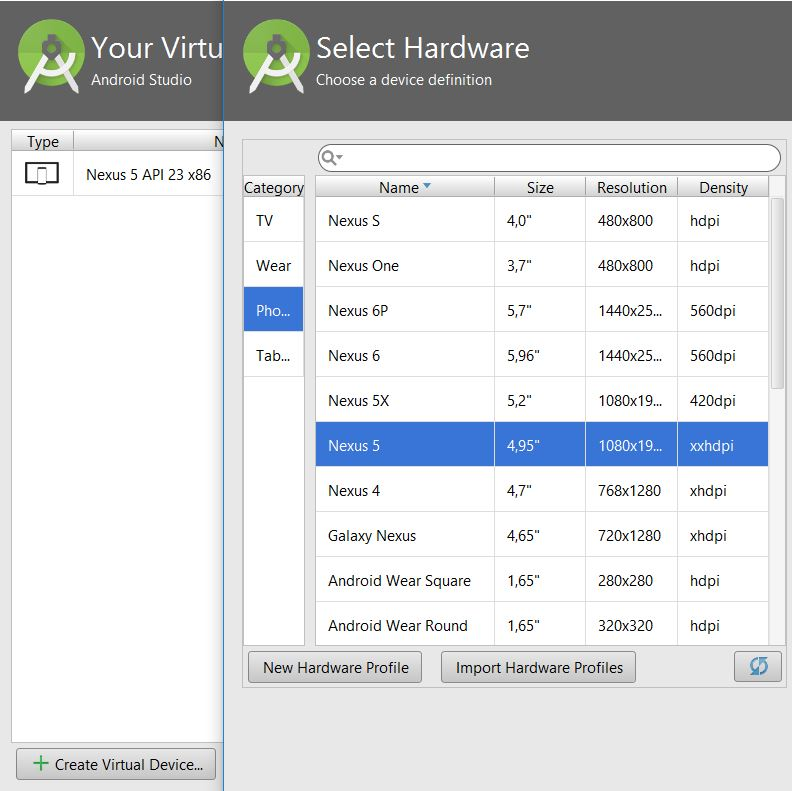
\includegraphics[width=0.4\textwidth]{images/Create-virtual-device}
	\caption{Erstellen einer AVD in Android Studio}
\end{wrapfigure}

\textbf{Android Virtual Device}
\begin{wrapfigure}{r}{0.3\textwidth}
	\centering
	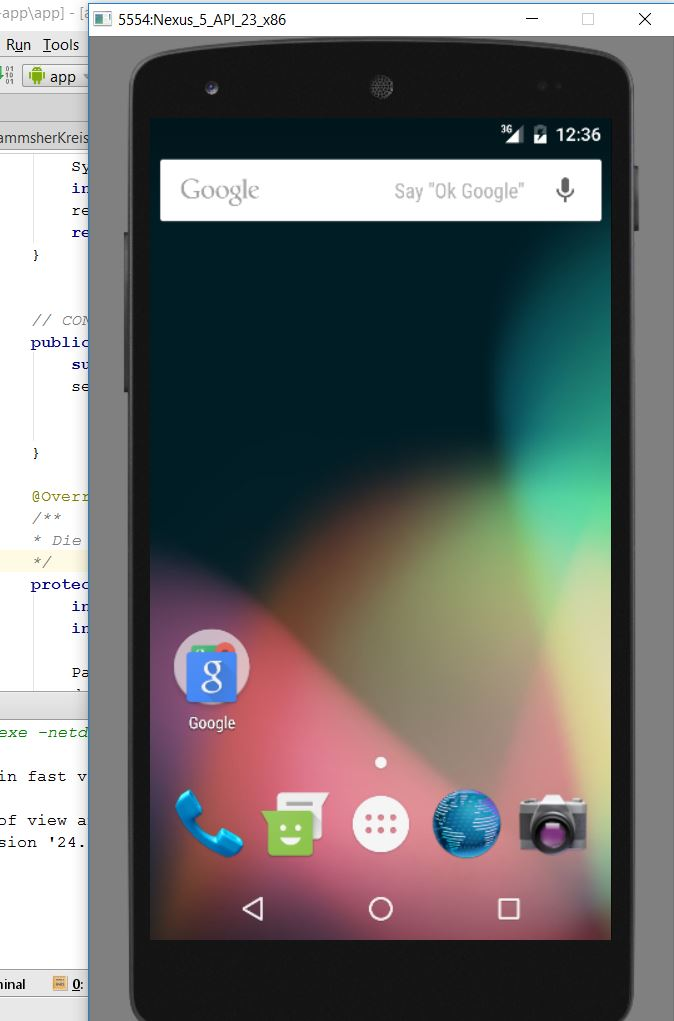
\includegraphics[width=0.4\textwidth]{images/AVD}
	\caption{AVD}
\end{wrapfigure}

\clearpage % DO NOT REMOVE